
\section{Feature descriptions, feature structures and models}

\subtitle{Feature descriptions, feature structures and models}

\huberlintitlepage[22pt]


\outline{

\begin{itemize}
\item Introduction and basic terms
\item Phrase structure grammar and \xbar Theory
\item Government \& Binding (GB)
\item {Generalized Phrase Structure Grammar (GPSG)}
\item \alert{Feature descriptions, feature structures and models}
\item Lexical Functional Grammar (LFG)
%\item PATR
\item Categorial Grammar (CG)
\item Head-Driven Phrase Structure Grammar (HPSG)
%\item Konstruktionsgrammatik (CxG)
\item Tree Adjoning Grammar (TAG)
\end{itemize}

%\tableofcontents
}

\frame{
\frametitle{Reading material}

\citew[Chapter~6]{MuellerGT-Eng}

}

%


\subsection{Feature descriptions}

\frame{
\frametitle{Feature descriptions and feature structures}

\alert{Feature structures} are used to model linguistic objects:
\begin{itemize}
\item attribut value structure
\item feature structure
\end{itemize}

Linguistis use \alert{feature descriptions} to talk about feature structures:
\begin{itemize}
\item attribute-value matrix (AVM)
\item feature matrix
\end{itemize}

\medskip
\pause
\begin{itemize}
\item \citet{Shieber86a}, \citet{ps}, \citet{Johnson88},\\%
      \citet{Carpenter92a}, \citet{King94a}, \citet{Richter2004a-u,Richter2021a}
\end{itemize}

}


\frame[shrink]{
\frametitle{An example}

A feature description, describing a human being:\\

\medskip
\scalebox{0.8}{\ms{
firstname    & max\\
lastname   & meier\\
date-of-birth & 10.10.1985\\
}
}

\medskip
\pause
Recursive descriptions:\\

\medskip
\scalebox{0.8}{\ms{
firstname    & max\\
lastname   & meier\\
date-of-birth & 10.10.1985\\
father      & \ms{
             firstname & peter\\
             lastname  & meier\\
             date-of-birth   & 10.05.1960\\
             father     & \ldots\\
             mother     & \ldots\\
             }\\
mother     & \ldots\\
}
}

\medskip
\pause
Exercise: How can we represent daughters or sons of a human being?

}


\iftoggle{loesungen}{

\subsubsection{Lists}

\frame{

\small
\frametitle{Solution I: Features\only<4->{, a lot of features}}


\scalebox{0.8}{\ms{
firstname    & max\\
lastname  & meier\\
date-of-birth & 10.10.1985\\
father      & \ldots\\
mother     & \ldots\\
daughter    & \ldots\\   
}}

\pause
What if we have several daughters?
\pause

\scalebox{0.8}{\ms{
firstname    & max\\
lastname  & meier\\
date-of-birth & 10.10.1985\\
father      & \ldots\\
mother     & \ldots\\
daughter-1    & \ldots\\   
daughter-2  & \ldots\\
daughter-3  & \ldots\\
}}

\pause
How many features do we want to assume? Where is the limit?\\
What is the value of \textsc{daughter-32}?

}

\frame{

\frametitle{Solution II: Lists}


\scalebox{0.75}{\ms{
firstname     & max\\
lastname      & meier\\
date-of-birth & 10.10.1985\\
father        & \ldots\\
mother        & \ldots\\
daughters     & \liste{ \ldots, \ldots }\\   
}}

\pause
What about sons?


\pause
Do we want to make this difference?\\
Yes, but the property is a property of the described objects:

\scalebox{0.75}{\ms{
firstname    & max\\
lastname   & meier\\
date-of-birth & 10.10.1985\\
\alert{gender} & \alert{male}\\
father      & \ldots\\
mother     & \ldots\\
\alert{children}  & \alert{\liste{ \ldots, \ldots }}\\   
}
}
}
}%\end{loesungen}

\subsubsection{Types}

\frame{
\frametitle{Types}

\begin{itemize}
\item Feature structures are of a certain type.
\item The type is written in \textit{italics}:

\ms[type]{ 
     A1 & V1 \\
}\\
\pause
\item Types specify which features have to belong to a certain feature structure.
\pause
\item Types are organized in hierarchies.

Example: part of speech\\
~\\[1ex]
\centerline{\mbox{\includegraphics{types-pos.eps}}}
\end{itemize}
}


\iftoggle{loesungen}{
\frame{
\frametitle{Feature descriptionen of type \type{person}}

\begin{itemize}
\item Our example description describes objects of type \type{person}.

\medskip
\scalebox{0.8}{
\ms[\alert{person}]{
firstname    & firstname\\
lastname & lastname\\
date-of-birth & date\\
gender & gender\\
father      & person\\
mother    & person\\
children    & list of person~
}
}

\medskip
\pause
\item Properties like \textsc{operating voltage} are irrelevant for such objects!

\pause
\item Type specifies which features are relevant for such an object.
\pause
\item We know: every human has a birthday even if we don't know the exact value.
\end{itemize}
}
}%\end{loesungen}

\subsubsection{Structure sharing}

\handoutframe{
\frametitle{Structure sharing}

Values of \textsc{A1} and \textsc{A2} are token-identical:

\ms{A1 & \ibox{1} \mbox{\rm [\textsc{A3}  \type{W3}]} \\
    A2 & \ibox{1} \\
   }

The identity of values is indicated by boxes.

Boxes are like variables or like pointers to some place in memory.

}


\iftoggle{loesungen}{
\frame{
\frametitle{Our example with children: One or two?}

\begin{itemize}
\item Do we describe one or two children of Peter and Anna?

\medskip
\scalebox{0.75}{\ms[person]{
firstname    & max\\
lastname   & meier\\
date-of-birth & 10.10.1985\\
father      & \ms[person]{
              firstname  & peter\\
              lastname & meier\\
              children   & \liste{ \ms[person]{
                                 firstname & \gruen{klaus}
                                 }, \ldots }
             }\\
mother    & \ms[person]{
              firstname  & anna\\
              lastname & meier\\
              children   & \liste{ \ms[person]{
                                 firstname & \gruen{klaus}
                                 }, \ldots }
             }
}
}
\medskip

\pause
\item We don't know!

\pause
\item There may be two different children from previous partnerships named \emph{Klaus}.
\end{itemize}
}


\frame{
\frametitle{Our example with children: Structure sharing}

\begin{itemize}
\item Do we describe one or two children of Peter and Anna?

\medskip
\scalebox{0.75}{\ms[person]{
firstname    & max\\
lastname   & meier\\
date-of-birth & 10.10.1985\\
father      & \ms[person]{
              firstname  & peter\\
              lastname & meier\\
              children   & \liste{ \ibox{1} \ms[person]{
                                 firstname & klaus
                                 }, \ldots }
             }\\
mother    & \ms[person]{
              firstname  & anna\\
              lastname & meier\\
              children & \liste{ \ibox{1}, \ldots }
             }
}}
\medskip

\pause
\item Klaus is a single child that belongs to both parents.
\pause
\item What about Max?
\end{itemize}
}

\subsubsection{Cyclic structures}

\frame{
\frametitle{Our example with children: Cyclic descriptions}


\begin{itemize}
\item \ibox{2} is placed in front of the description and occurs within it.

\medskip
\scalebox{0.95}{
\ibox{2} \ms[person]{
firstname    & max\\
lastname   & meier\\
date-of-birth & 10.10.1985\\
father      & \ms[person]{
              firstname  & peter\\
              lastname & meier\\
              children   & \liste{ \ibox{1} \ms[person]{
                                 firstname & klaus
                                 }, \ibox{2} }
             }\\
mother    & \ms[person]{
              firstname  & anna\\
              lastname & meier\\
              children   & \liste{ \ibox{1}, \ibox{2} }
             }
}
}
\end{itemize}

\vfill

}


}%\end{loesungen}

\subsubsection{Unification}

\frame{
\frametitle{Unification}

\begin{itemize}[<+->]
\item Grammatical rules \& lexical items are described by feature descriptions.
\item Grammatical rules contain partial descriptions of daughters,\\
      but not the complete information.
\item A specific phrase has to be compatible with the demands regarding the daughter to be able to
  enter the structure.
\item Term for this specific kind of compatibility: \alert{unifyability}
\item When two structures are unified, the result is a new structure containing all information of
  the two unified structures and nothing more.
\end{itemize}


}

\frame{
\frametitle{Example: Detective agency}

\begin{itemize}
\item We are searching for a blond, female person named Meier.
\pause
\item A possible description:\\
\medskip
\ms[person]{
lastname   & meier\\
gender & female\\
haircolor  & blonde
}

\medskip

\pause
\item If we get a search result matching the following description,\\
      we change the agency.

\medskip
\ms[person]{
lastname   & meier\\
gender & \rot{male}\\
haircolor & \rot{red}
}

\end{itemize}

}

\frame{
\frametitle{Example: Detective agency}
%\smallframe

\begin{itemize}
\item We are searching for a blond, female person named Meier.

\medskip
\scalebox{0.9}{\ms[person]{
lastname   & meier\\
gender & female\\
haircolor  & blonde
}}

\medskip
a possible result:

\medskip
\scalebox{0.9}{\ms[person]{
firstname    & katharina\\
lastname   & meier\\
gender & female\\
date-of-birth & 15.10.1965\\
haircolor  & blonde
}}

\medskip
\pause
\item Katharina Meier may have further properties unknown to the detective.

Important: those he does know have to be compatible to the request.

\end{itemize}

}

\frame{
\frametitle{Example: Detective agency}

\begin{tabular}{@{}l@{\hspace{2em}}l@{}}
The unification of the request & with the information of the detective\\[2mm]
\scalebox{0.85}{\ms[person]{
lastname   & meier\\
gender & female\\
haircolor  & blonde\\
}} & \scalebox{0.85}{\ms[person]{
firstname    & katharina\\
lastname   & meier\\
gender & female\\
date-of-birth & 15.10.1965\\
haircolor  & blonde\
}}\\
\\
\multicolumn{2}{@{}l@{}}{%
\alt<beamer>{is \visible<2>{but \rot{not}:}}{is not the following, since he does not have any information about children:}}\\[2mm]
\scalebox{0.85}{\ms[person]{
firstname    & katharina\\
lastname   & meier\\
gender & female\\
date-of-birth & 15.10.1965\\
haircolor  & blond\\
\visible<2>{\rot{children}} & \visible<2>{\rot{\liste{}}}\\
}} & \begin{tabular}{@{}l@{}}
     \visible<2>{The detective may not invent properties!}\\
     \visible<2>{He risks his job}\\
     \visible<2>{by providing possibly wrong information!}\\
     \end{tabular}
\end{tabular}

}

\subsection{Phenomena, models and formal theories}

\frame{
\frametitle{Phenomena, models and formal theories}

\vfill

\hfill
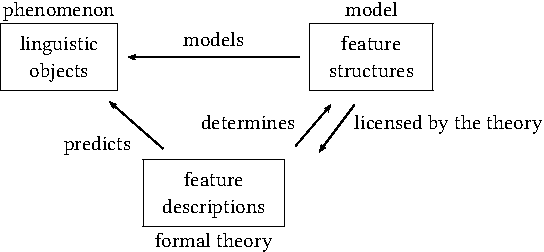
\includegraphics{Figures/model-theory-phenomenon-crop}
\hfill\hfill\mbox{}

\vfill

}



\subsection{Homework}

\frame[shrink=15]{
\frametitle{Homework}

\begin{enumerate}
\item Think about how one could describe musical instruments using feature descriptions.
\item Come up with a type hierarchy for the word classes (\type{det}, \type{comp}, \type{noun}, \type{verb},
      \type{adj}, \type{prep}). Think about the ways in which one can organize the type hierachy so that one
	  can express the generalizations that where captured by the binary features in on slide~\ref{slide-lex-kat-gb}.
\item\label{ua-liste} I motivated the introduction of lists. This may look like an extension of the formalism, but it is not as it is possible to
convert the list notation into a notation which only requires feature"=value pairs. Think about how one could do this.
\item (Additional exercise) The relation \emph{append}\is{relation!\emph{append}} will play a role
  in the introduction of HPSG. This relation serves to
combine two lists to form a third.
Relational constraints such as \emph{append} do in fact constitute an expansion of the formalism. Using relational constraints, it is possible to relate any number
of feature values to other values, that is, one can write programs which compute a particular value depending on other values. 
This poses the question as to whether one needs such powerful descriptive tools in a linguistic theory and if we do allow them, what kind of complexity we afford them.
A theory which can do without relational constraints should be preferred over one that uses
relational constraints (see \citealp[Chapter~20]{MuellerLehrbuch} for a comparison of theories).

For the concatenation of lists, there is a possible implementation in feature structures without
recourse to relational constraints. Find out how this can be done. Give your sources and document
how you went about finding the solution.
\end{enumerate}

}


%      <!-- Local IspellDict: en_US-w_accents -->
